\documentclass{article}
\usepackage{amsmath,amssymb,amsbsy,amsfonts,amsthm}
\usepackage{graphics,epsfig,graphicx,float,subfigure,color}
\usepackage{url}
\usepackage{float}

\title{State Estimation with Kalman Filtering applied to Reinforcement Learning}
\author{Abraham Frei-Pearson \\
	Department of Mathematics  \\
	\and 
	Sheroze Sheriffdeen \\
	Oden Institute \\
	}

\date{\today}
% Hint: \title{what ever}, \author{who care} and \date{when ever} could stand 
% before or after the \begin{document} command 
% BUT the \maketitle command MUST come AFTER the \begin{document} command! 
\begin{document}

\maketitle

\section{Kalman Filtering for State Estimation}
\subsection{Discrete Time-Controlled Processes}

For this section of our project, we are interested in applying reinforcement learning techniques to noisy optimal control problems. The general case will be in the following form. Given a $A \in \mathbb{R}^{n \times n}$, $B \in \mathbb{R}^{n \times n_u}$, the state will be a vector $x_t \in \mathbb R^n$, and our dynamics will be governed by the linear stochastic difference equation
\begin{equation}
    x_{t+1} = (I + \triangle t A) x_t + Bu(x_t) + w_t,
    \label{eq:dynamical}
\end{equation}
with state measurements,
\[
	z_{t+1} = H x_{t+1} + v_{t+1}
\].
The random variables $w_t$ and $v_t$ represent process and measurement noise respectively. They are assumed to be independent of each other, white, with normal probability distributions
\[ 
p(w) \sim \mathcal{N}(0, Q)
\]
\[
p(v) \sim \mathcal{N}(0, R)
\]

$u(x_t) \in \mathbb{R}^{n_u}$ is the control vector that we are trying to learn using reinforcement learning. We employ true-online TD($\lambda$) to learn a parametrized control vector at each time step given noisy measurements of state.

\subsection{State Estimation with Kalman Filtering}

The following is from the excellent introduction to Kalman filters by Welch and Bishop \cite{welch1995introduction}. The Kalman filter is a set of mathematical equations that provide efficient means of estimating the state of a physical process given observations. At each step, an \textit{a priori} estimate of the state $\hat{x}_{t}^{\text{p}}$ represents the knowledge of the process state prior to time $t$. The controller, or the reinforcement learning algorithm, picks a parametrized action given this prior estimate. The action is then executed, and a noisy observation of the state is obtained from the environment. This observation is used to compute an \textit{a posteriori} estimate of the state $\hat{x}_{t}$. We can then define $\textit{a priori}$ and $\textit{a posteriori}$ estimate errors as,
\begin{align*}
	e^{\text{p}}_t &= x_t - \hat{x}_{t}^{\text{p}} \\
	e_t &= x_t - \hat{x}_{t} 
\end{align*}

The estimate error covariances are,
\begin{align}
	P^p_t &= \mathbb{E}\left[e^{\text{p}}_t e^{\text{p}T}_t \right]  \\
	P_t &= \mathbb{E}\left[e_t e_t^{T} \right] \label{eq:ap_err_cov}
\end{align}

The Kalman filter begins with the goal of finding an equation that computes the a posteriori state estimate as a linear combination of the a priori estimate and an affine function of the difference between the actual measurement and the predicted measurement.
\begin{equation}
	\hat{x}_t = \hat{x}_t^p + K(z_t - H\hat{x}_t^p)
	\label{eq:ap}
\end{equation}
The difference $(z_t - H\hat{x}_t^p)$ is called the measurement innovation, or the residual.  $K \in \mathbb{R}^{n \times n_u}$ is the gain that minimizes the a posteriori error covariance (\ref{eq:ap_err_cov}). One form of the resulting K \cite{maybeck1982stochastic} is, 
\begin{equation}
	K_t = P_t^p H^T(HP_t^pH^T + R)^{-1}
	\label{eq:k_gain}
\end{equation}
As measurement error covariance $R$ approaches zero, the gain approaches the inverse of the measurement operator $H^{-1}$. 

\subsubsection{Kalman Filter Prediction-Correction}
Given a policy $\pi$, the following steps outline a robust method to pick actions by employing state estimation. 

Initialize Kalman filter with $\hat{x}_0$ to the initial state. Assume $A, B, P, Q, H$ are known. For each $t = (1, \ldots, T)$, 
\begin{enumerate}
	\item Pick action $a_{t-1} \sim \pi(\cdot | \hat{x}_{t-1})$. 
	\item Map from action to parametrized control vector $u_{t-1}$.
	\item Obtain a priori estimate of state: $\hat{x}_t^p = A\hat{x}_{t-1} + Bu_{t-1}$.
	\item Project covariance estimate forward in time: $P_{t}^p = AP_{t-1}A^T + Q$.
	\item Compute Kalman gain $K_t$ from equation (\ref{eq:k_gain}).
	\item Take action $a_t$ and evolve dynamical system according to (\ref{eq:dynamical}) to obtain measurement $z_t$.
	\item Compute a posteriori estimate of state using (\ref{eq:ap}).
	\item Update covariance estimate $P_t = (I - K_tH)P_t^p$.
\end{enumerate}

Using the a posteriori estimate for the state gives a mechanism to perform policy evaluation and control by using the Kalman filter as the mediation between the measurements obtained from the environment and the internal representation of the state. Furthermore, for cases where the discrete-time controlled process is governed by a nonlinear stochastic difference equation, a Kalman filter that linearizes around the current mean and covariance referred to as an extended Kalman filter can be used to obtain robust estimates of the state. This report focuses only on the linear dynamical system case.

\subsection{Experiment}

The following experiment we uses true online Sarsa($\lambda$) to estimate $q^*$ as described in \cite{sutton2018reinforcement} for a linear dynamical system. State-action feature vector with tile coding $x = x(s, a)$ is used to encode the 2-dimensional continuous state space $[-2, 2] \times [-2, 2] \subset \mathbb{R}^2$. 10 tilings were used with tile width $= [0.1, 0.1]$. The Q-function is then parametrized as $q(s, a, w) = w^Tx(s,a)$. The values describing the linear dynamical system in (\ref{eq:dynamical}) is as follows:
\[
A = \begin{bmatrix}
0 & 1 \\
1 & 1
\end{bmatrix}, \quad 
B = \begin{bmatrix}
\eta & 0 \\
0 & \eta
\end{bmatrix}, \quad
H = \begin{bmatrix}
1 & 0 \\
0 & 1
\end{bmatrix}, \quad
Q = \begin{bmatrix}
q & 0 \\
0 & q
\end{bmatrix}, \quad
R = \begin{bmatrix}
r & 0 \\
0 & r
\end{bmatrix}
\]
with $\triangle t = 0.02$, $q = 10^{-7}$, $\eta = 0.02$,  and $r$ varied from $10^{-3}$ to $10^{-8}$ to determine the effect of measurement noise on policy control with and without state estimation with Kalman filtering. The map $x_t = Ax_{t-1}$ has a hyperbolic fixed point with eigenvalues,
\begin{align*}
	\lambda_1 &= \dfrac{3 + \sqrt{5}}{2} \\
	\lambda_2 &= \dfrac{3 - \sqrt{5}}{2}
\end{align*}
\begin{figure}[H]
	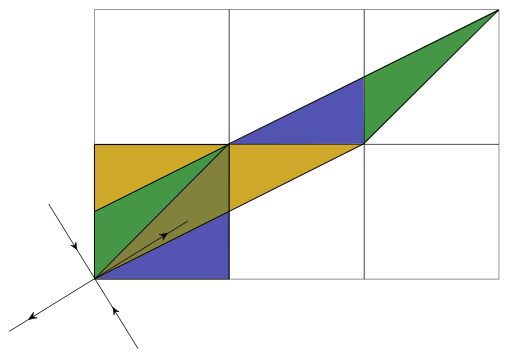
\includegraphics[scale=0.5]{Arnoldcatmap.png}
	\caption{The lines with the arrows show the contracting and expanding eigenspaces. The control should force the state to straddle the contracting eigenspaces to reach the hyperbolic equilibrium point.  \texttt{https://commons.wikimedia.org/wiki/File:Arnoldcatmap.svg} }
\end{figure}
The actions were parametrized to limit the control to act only in the $x$-direction with the options being move left, right, and no control with corresponding control vectors being $[-1, 0], [1, 0], [0,0]$. The initial condition was chosen to be within a 2-D ball of radius 0.05 centered at $[-1.62, 1]$ which lies on the contracting eigenspace. The terminal states are the cases where the state reaches failure regions defined to be $b$ away from the contracting eigenspaces (below the line $y = \dfrac{-2x}{1+\sqrt{5}} - b$ and above the line $y = \dfrac{-2x}{1+\sqrt{5}} + b$). If the controller is successful in containing the state to be within the success region for 400 time steps, a terminal state is reached. For each time step in the success region, a reward of $+1$ is received. 



\bibliographystyle{plain} 
\bibliography{references}

\end{document}
